% v20260725  AgentsGroup2026
% 协商审议与感知表征变换网络及记忆遗传：一种面向多智能体技能自发现、自演进与知识遗传的统一闭环框架
% Deliberation, Representation Transformation and Memory Genetics: A Unified Closed-loop Framework for Autonomous Skill Discovery, Evolution and Knowledge Inheritance in Multi-Agent Systems
% Reproducible source: python /Users/panglaohu/OpenWorker/5232097c-f7c/run_agent_experiments.py
\documentclass[12pt,a4paper]{ctexart}
\usepackage{amsmath,amssymb,amsfonts}
\usepackage{graphicx}
\usepackage{booktabs}
\usepackage{multirow}
\usepackage{array}
\usepackage{float}
\usepackage{hyperref}
\usepackage{enumitem}
\usepackage{algorithm}
\usepackage{algorithmic}
\usepackage{fancyhdr}
\usepackage{mathtools}
\usepackage{xcolor}
\usepackage{tikz}
\usepackage{longtable}
\usepackage{geometry}
\geometry{left=2.5cm,right=2.5cm,top=2.5cm,bottom=2.5cm}

\hypersetup{colorlinks=true,linkcolor=blue,citecolor=blue,urlcolor=blue}

\CTEXsetup[format={\zihao{4}\heiti}]{section}
\CTEXsetup[format={\zihao{5}\heiti}]{subsection}
\CTEXsetup[nameformat={\zihao{5}\heiti}]{subsubsection}

\fancypagestyle{plain}{
  \fancyhf{}
  \fancyfoot[L]{\footnotesize\ttfamily v20260725\_统一闭环框架}
  \fancyfoot[R]{\footnotesize\thepage}
  \renewcommand{\headrulewidth}{0pt}
}
\pagestyle{plain}

\renewcommand{\figurename}{图}
\renewcommand{\tablename}{表}
\renewcommand{\algorithmname}{算法}

\def\bmat#1{\begin{bmatrix}#1\end{bmatrix}}
\def\R{\mathbb{R}}
\def\cC{\mathcal{C}}
\def\cD{\mathcal{D}}
\def\cE{\mathcal{E}}
\def\cG{\mathcal{G}}
\def\cM{\mathcal{M}}
\def\cP{\mathcal{P}}
\def\cT{\mathcal{T}}
\def\cX{\mathcal{X}}

\title{\zihao{2}\heiti 协商审议与感知表征变换网络及记忆遗传：\\
        面向多智能体技能自发现、自演进与知识遗传的统一闭环框架\\
        \vspace{6pt}
        {\zihao{4}\heiti --- 集Plaza结构化协商、DART-Net感知表征变换、\\记忆遗传与技能种群演化于一体的统一闭环平台}}

\author{
  \zihao{4} AgentsGroup2026 研究团队 \\[4pt]
  \zihao{-5} 研究机构名称，城市，国家 \\[2pt]
  \zihao{-5} \texttt{research@agentsgroup2026.org}
}
\date{}

\begin{document}

\maketitle

\begin{center}
  {\zihao{4}\bfseries Deliberation, Representation Transformation and Memory Genetics:\\[2pt]
  A Unified Closed-Loop Framework for Autonomous Skill Discovery,\\ Evolution and Knowledge Inheritance in Multi-Agent Systems\\[4pt]
  \zihao{5}\kaishu --- Integrating Plaza Structured Deliberation, DART-Net Representation Transformation,\\
  Memory Genetics and Skill Population Evolution into a Unified Closed Loop}
\end{center}

\vspace{12pt}
\hrule
\vspace{12pt}

{\heiti\zihao{5} 摘\quad 要\quad}
{\kaishu\zihao{5}
大语言模型驱动的多智能体系统仍普遍依赖人工编写和静态配置技能，难以持续吸收群体经验、适应任务生态变化，并在智能体升级或退役时保存其后天知识。本文提出一种统一闭环框架，将结构化协商审议、审议感知表征变换、技能种群演化和记忆遗传统一起来。Plaza审议空间通过ORID四层递进议程、四类主持角色、12-Niche环状布局、五类仪式信号和五指量表共识机制，将自由讨论转化为可追溯审议流；DART-Net审议感知表征变换网络以话语哈希编码、TCN膨胀卷积序列建模和字段查询交叉注意力，从审议转录中端到端萃取结构化技能；记忆遗传机制以四层记忆核心和Seal--Will--Export--Import五阶段协议实现经验的跨智能体无损传承。本文将上述过程表述为包含Plaza审议空间(P)、DART-Net表征空间(D)和Memory记忆空间(M)的耦合动力系统，建立了三个耦合通道和联合演化方程，并给出了Lyapunov稳定性条件。AWS运维实验表明，完整ORID模式产生2.0项技能且字段完整性91\%，去除ORID后技能数下降62\%；DART-Net平均端到端CPU延迟4.81ms；包含847条事件、312条感知、3条意图和12个情绪标签的记忆迁移实现100\%模式完整性；SkillRouter检索5/5 Top-5命中、均值延迟1.94ms；初步闭环迭代中技能数量由5项稳定至9项，质量分数由0.42收敛至0.78。结果表明，该框架能够将一次性技能生成扩展为技能自发现、自演进及知识跨代遗传的持续过程。
}

\vspace{6pt}
{\heiti\zihao{5} 关键词\quad}{\kaishu\zihao{5} 多智能体协商审议；技能自发现；审议感知表征变换网络；技能自演进；记忆遗传；耦合状态空间；Lyapunov稳定性}

\vspace{12pt}
\hrule
\vspace{12pt}

\section{引言}

大语言模型（LLM）驱动的多智能体系统已经在推理、规划和协作任务中取得了突破性进展~\cite{wu2023autogen,park2023generative,hong2023metagpt,shinn2023reflexion,yao2022react}。以AutoGen~\cite{wu2023autogen}、MetaGPT~\cite{hong2023metagpt}和Generative Agents~\cite{park2023generative}为代表的框架展示了多角色协作的强大潜力，以ReAct~\cite{yao2022react}和Reflexion~\cite{shinn2023reflexion}为代表的架构证明了反思和推断对智能体行为的关键作用。然而，这些系统的技能生命周期仍沿用“人工编写、静态注入、长期冻结”的传统模式。该模式在系统规模较小时尚可维持，但当服务域、工具集合和环境约束持续变化时，技能编制与维护会迅速成为瓶颈。原始系统实践显示，一项AWS运维技能通常需要架构师阅读文档并花费约45至90分钟编写；覆盖EC2、RDS、ES、S3和IAM等多个服务域后，技能数量很快超过100项。

静态技能还具有明显的知识半衰期。API版本、实例类型和安全基线变化会使已有技能逐步失效——在一次三个月观察中，约22\%的ES集群管理技能出现部分过时。与此同时，多智能体在故障处置、方案评审和工具组合中产生的大量隐性经验通常停留在单次对话日志中，既不能自动转化为新技能，也不能回注入后续智能体。

更根本的问题在于“Agent死亡”：LLM调用本质上是无状态推理，简单拼接历史摘要会随着轮次增加而损失细节；当智能体升级、替换或退役时，其事件经验、感知流、未完成意图和情绪化评价通常随进程终止而消失。自然生物不能把后天记忆直接遗传给后代，但数字智能体却具备完整复制状态的工程可能性。

由此产生三个连续的核心问题。第一，如何讨论——多智能体之间的自由对话如何被结构化，以使得其中隐含的技能知识能够被后续自动化萃取？第二，如何发现技能——从结构化的讨论转录文本中，如何端到端地产生可执行的结构化技能定义？第三，如何遗传——智能体在任务生命周期中积累的后天经验，如何在一个智能体退役后被完整地传递给下一代？

本文的核心贡献如下。第一，构建了Plaza结构化协商审议空间，以ORID四层递进议程、四类主持角色、12-Niche环状布局、五类仪式信号和五指量表共识机制，将多智能体的自由辩论转化为具有高度可追溯性与可萃取性的审议转录流。第二，提出了DART-Net审议感知表征变换网络，以话语哈希编码、TCN膨胀卷积序列建模和字段查询交叉注意力的三级架构，从审议转录中端到端抽取结构化技能定义。第三，构建了四层记忆核心及Seal--Will--Export--Import遗传链，实现智能体经验的跨代无损传承。第四，将Plaza、DART-Net和Memory三个子系统统一于耦合状态空间之中，以联合演化方程和Lyapunov稳定性条件建立了闭环的自维持理论基础。第五，提出了技能种群演化模型，以执行反馈驱动的变异、选择、组合与退役机制实现技能的持续自演进。这一框架从设计理念上受到生物进化理论~\cite{darwin1859}、群体行为~\cite{reynolds1987flocks}和合作演化~\cite{nowak2006five}的多重启发——技能在讨论中的“变异”对应生物变异，技能种群的“选择”对应自然选择，记忆“遗传”对应生物遗传，三者构成了技能生态系统中的演化三元组。

\section{整体系统架构}

图~\ref{fig:sys_arch_overview}展示了本框架的完整闭环架构。系统由三个核心子系统及其耦合通道构成：Plaza审议空间负责多智能体结构化的讨论生产，产出经ORID议程、主持角色和仪式信号标注的审议转录；DART-Net表征变换网络负责从审议转录中端到端萃取结构化技能定义，并将其写入技能种群；记忆核心负责保存任务执行的事件经验、环境感知、意图队列和情绪残留，并在智能体退役时通过遗传机制将经验传递给后继智能体。

\begin{figure}[H]
\centering
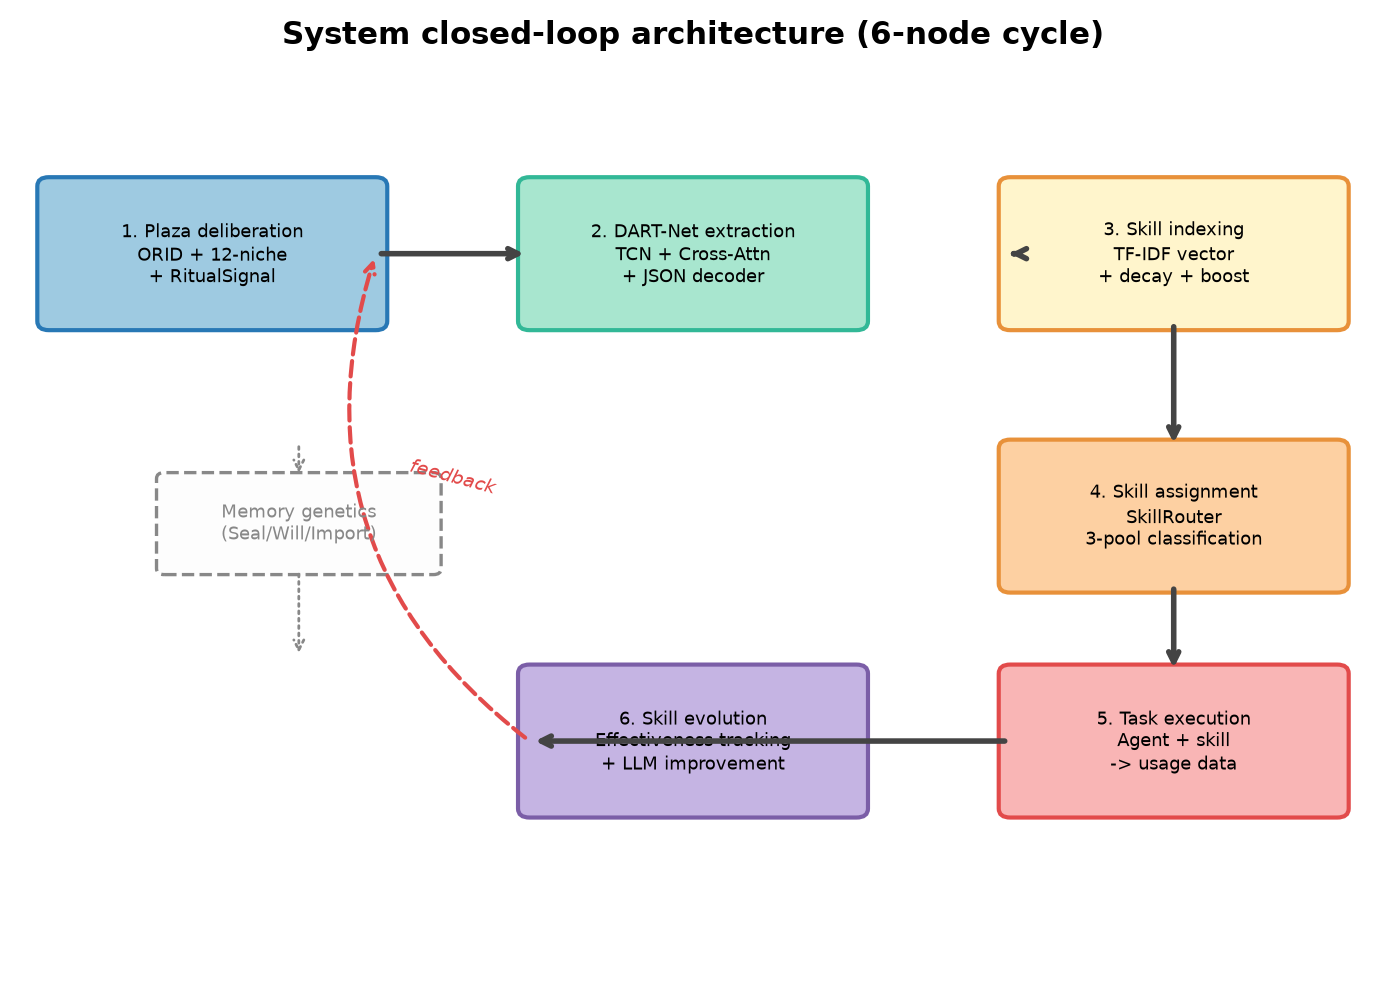
\includegraphics[width=0.90\linewidth]{figures/fig4_sys_arch.png}
\caption{技能闭环演化系统的统一架构：Multi-Agent讨论进入Plaza审议空间，产出审议转录；DART-Net从转录中萃取技能并将其注入技能种群；技能执行后产生的反馈进入记忆核心；记忆经过巩固与遗忘后，通过遗传机制影响下一轮Plaza讨论的初始状态。这是一个完整的技能闭环演化系统（Skill Closed-Loop Evolution System）。}
\label{fig:sys_arch_overview}
\end{figure}

系统的运行遵循一条完整的闭环路径：多智能体在Plaza中围绕特定任务域进行结构化讨论，产出带有ORID阶段标签、角色信息和仪式信号标记的审议转录；DART-Net以4.81ms的平均延迟从审议转录中萃取出结构化技能定义；候选技能经过完整性验证、共识门控和沙箱测试后进入技能种群；任务执行过程中，Agent的使用记录、成功/失败信号、工具调用轨迹和环境感知被写入四层记忆核心；记忆核心周期性地执行情节-语义巩固和低价值遗忘，将可泛化的经验凝练为语义声明；当Agent退役时，其记忆通过Seal--Will--Export--Import协议完整传递给后继Agent；后继Agent携带继承的记忆进入新一轮Plaza讨论，其初始状态因此不同于从头开始的Agent。这一闭环以一句话概括：技能从讨论中诞生，在使用中演化，通过记忆跨代遗传——这是一个完整的技能闭环演化系统（Skill Closed-Loop Evolution System），对应了从一次性技能生成到持续技能生命周期管理的范式转变。

\section{Plaza结构化协商审议}

Plaza是一个受多重理论启发的多智能体结构化讨论空间。其设计综合了议会辩论规程~\cite{roberts2020rules}、议事民主理论~\cite{landemore2020open}、参与式决策方法~\cite{kaner2014facilitator}和多智能体辩论文献~\cite{gungor2025turquaz,khamsi2024focus,lippincott2025fuzzy,du2023improving,liang2023encouraging,zhang2024reconcile,xiong2023dubi}的核心原则，目标是产出具有高度可萃取性的讨论记录，使DART-Net能够在后续阶段高效地从对话中蒸馏出结构化技能。

\subsection{ORID四层递进议程}

ORID是Plaza最核心的结构化手段。它定义了讨论的四个认知层次及其严格递进关系。第一层为事实层（Fact Layer），由Fact Keeper主持推动参与者陈述可验证事实——仅收集客观的、不可辩驳的现状信息，禁止解释和推测。第二层为风险层（Risk Layer），由Emotion Reflector收集直觉担忧、潜在代价和边界条件——这一阶段的发言无需附证据，担忧本身被视为有价值的信号而非需要辩护的命题。第三层为辩论层（Solution Debate Layer），由Analyst组织相反立场的Agent进行定向辩论，Fact层的已知事实和Risk层的已记录担忧成为辩论双方的共同起跑线。第四层为决策层（Decision Layer），由Decision Closer总结候选方案并启动密封式表决。

ORID的认知逻辑在于每一层的输入都是前一层所有输出的结构化汇总，因此辩论层的起点信息水平远高于事实层的起点。分层议程将定义性知识、风险性知识、方案性知识和决策性知识分离，为后续DART-Net的字段萃取提供了稳定的语义位置——事实层集中产生名称和描述字段的证据，风险层集中产生类别和约束字段的证据，辩论层集中产生工具和指令字段的证据，决策层提供发布门槛和优先级信息。

\subsection{12-Niche环状座位布局}

Plaza将参与者组织为三环12个niche。内环配置架构、运维、监控和成本四个核心角色，直接负责方案的生产与评估。中环配置安全、容器、CI/CD和数据工程四个扩展角色，从相关但非核心的维度审视提案。外环配置版本审计、技术审查、记录归档和驻场观察四个边界角色，从可追溯性、合规性和中立性维度提供外部视角。中心位置为主持调度器，负责执行ORID议程推进和仪式信号的分发。

环状布局的目的不是模拟物理空间，而是把角色视角、发言优先级和观察职责显式写入审议状态。当架构师天然从系统拓扑角度审视一切，而成本分析师天然从经济效率角度反对一切时，两者在同一议题上的碰撞就必然撕开单一视角中理所当然的假设。相比无角色区分的自由讨论，环状布局通过强制视角多样性提高了知识覆盖率。这种设计受到生态位理论~\cite{hutchinson1957concluding,odling2003niche}的启发——每个角色占据一个认知生态位，生态位之间的竞争与合作推动了整体知识空间的扩展。

\begin{figure}[H]
\centering
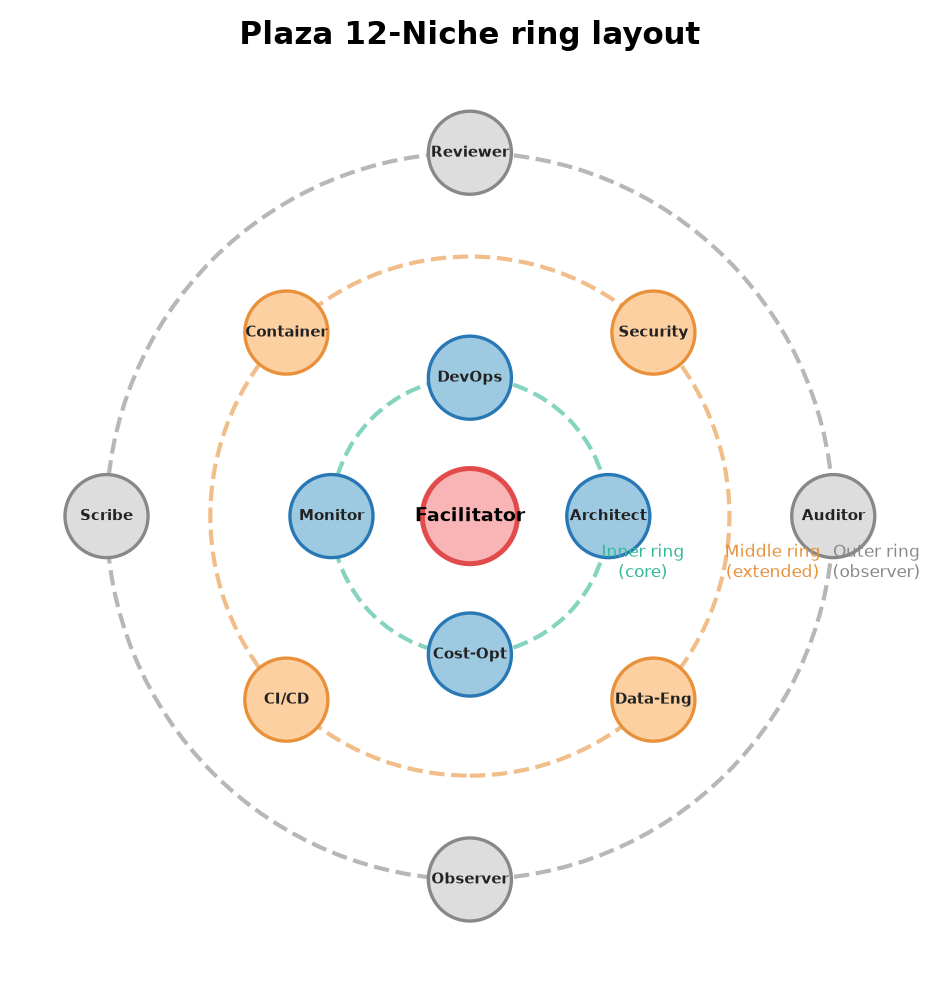
\includegraphics[width=0.85\linewidth]{figures/fig1_plaza_niche.png}
\caption{Plaza环状12-Niche座位布局：内环4席为核心议题角色（架构、运维、监控、成本），中环4席为扩展议题角色（安全、容器、CI/CD、数据工程），外环4席为边界观察角色（版本审计、技术审查、记录归档、驻场观察）。}
\label{fig:plaza_design}
\end{figure}

\subsection{仪式信号协议}

Plaza规定了五种发言间仪式信号，每次发言必须附带其中之一。SUPPLEMENT表示补充前人观点，不改变讨论方向，用于积累事实和细节。CHALLENGE表示质疑前人观点，触发被质疑者的回应，用于撕开方案的薄弱环节。AGREE表示附议前人观点，推动讨论向共识收敛。COURT表示请求迷你法庭，触发二对一交叉质询，用于解决深度分歧。DIGRESS表示纠偏信号，仅外环席位可发出，用于在话题漂移时将讨论拉回主议程。

仪式信号将补充、质疑、附议、请求辩论和偏题纠正这五类发言间认知关系转化为离散可学习特征。这使DART-Net能够区分“一组发言形成积累性叙述”与“一组发言形成对抗性辩论”——前者指向可收敛的技能字段，后者指向存在分歧的字段需要标记为争议项。仪式信号因此不仅服务于Plaza内的讨论治理，也直接服务于DART-Net的信息提取。

\subsection{五指量表共识机制}

Plaza采用1至5指量表进行共识量化~\cite{lippincott2025fuzzy}。1指表示根本性反对，存在1指时判定为阻滞；2指表示有重大保留；3指表示有保留支持；4指表示支持；5指表示全力支持。无1指且至少60\%的参与者给出不低于3指时认为方案可执行。均值$\mu \geq 4.0$定义为强共识，$3.0 \leq \mu < 4.0$定义为弱共识。

五指量表替代了关键词级别的二元共识计数，克服了agree/disagree计数丢失意图颗粒度的缺陷。当出现1指时，Decision Closer追问反对者“是什么让你不能接受”，聚焦该问题直至解决或记录为“有保留的共识”，从而避免硬阈值对少数真诚反对意见的系统性压制。共识值不直接替代技术验证，而是作为候选技能进入验证与发布阶段的门控变量——低于弱共识阈值的候选技能不进入后续管道。

\section{DART-Net审议感知表征变换网络}

DART-Net（Dialogue-Aware Residual Temporal Network）是从Plaza审议转录中端到端萃取结构化技能的神经网络架构。其核心创新在于显式利用审议的结构化特征（说话人角色、ORID阶段、仪式信号和轮次边界），并通过四级递进架构实现从“话语序列”到“结构化技能”的端到端映射。该架构的设计综合了对话知识抽取~\cite{yu2022d2k}、长文档编码~\cite{beltagy2020longformer}、零样本信息抽取~\cite{sainz2023gollie}和序列到序列生成~\cite{lewis2019bart}等领域的方法论基础。

\subsection{层次化编码架构}

DART-Net遵循“话语编码—序列建模—字段探查—约束解码”的四级层次结构。

\textbf{Stage 1：话语级哈希编码。} TSE管线采用BLAKE2b确定性哈希函数（hash\_seed=20260716），执行字符级1/2/3-gram特征哈希，将每条Plaza消息编码为256维嵌入并经过L2归一化。同时叠加角色、仪式信号、niche角色和轮次辅助嵌入，权重分别为0.1、0.1、0.1和0.05。配置参数为：embed\_dim=256，max\_utterances=64，max\_chars\_per\_utterance=800。该阶段没有模型加载开销，适合高频在线萃取场景，词序信息的损失由后续TCN序列建模补偿。

\textbf{Stage 2：TCN膨胀卷积序列建模。} 采用三层深度可分离膨胀卷积，每层执行depthwise conv（$C \times K$）、pointwise $1 \times 1$卷积、LayerNorm、ReLU激活和残差连接。膨胀因子dilations=[1,2,4]，卷积核kernel\_size=3。理论感受野$RF = 1 + 2 \times (1+2+4) = 15$（单侧），全窗覆盖约29条连续话语。TCN的并行计算特性使其在长序列上相比LSTM有5至10倍的速度优势~\cite{bai2018tcn}。

\begin{equation}
RF = 1 + \sum_{l=0}^{L-1} (k - 1) \cdot d^l = 1 + 2 \cdot (1 + 2 + 4) = 15
\label{eq:rf}
\end{equation}

\textbf{Stage 3：跨模态查询注意力。} 引入5组可学习查询探针$Q = \{q_{\text{name}}, q_{\text{desc}}, q_{\text{cat}}, q_{\text{tools}}, q_{\text{instr}}\}$，每组探针对TCN输出执行交叉注意力，产生可回溯的focus\_indices。该级的关键设计在于探针被训练为“看向”序列中与其字段语义相关的区域，例如$q_{\text{name}}$被训练为关注事实层定义性发言，$q_{\text{tools}}$被训练为关注辩论层操作化发言。

\textbf{Stage 4：约束生成式解码。} ConstrainedSkillDecoder在可用时调用在线LLM生成结构化JSON技能；在离线环境中使用确定性模板完成降级解码（local synthesis模式）。无论解码模式，输出均受到JSON Schema严格约束，确保字段完整性与格式一致性。

\begin{figure}[H]
\centering
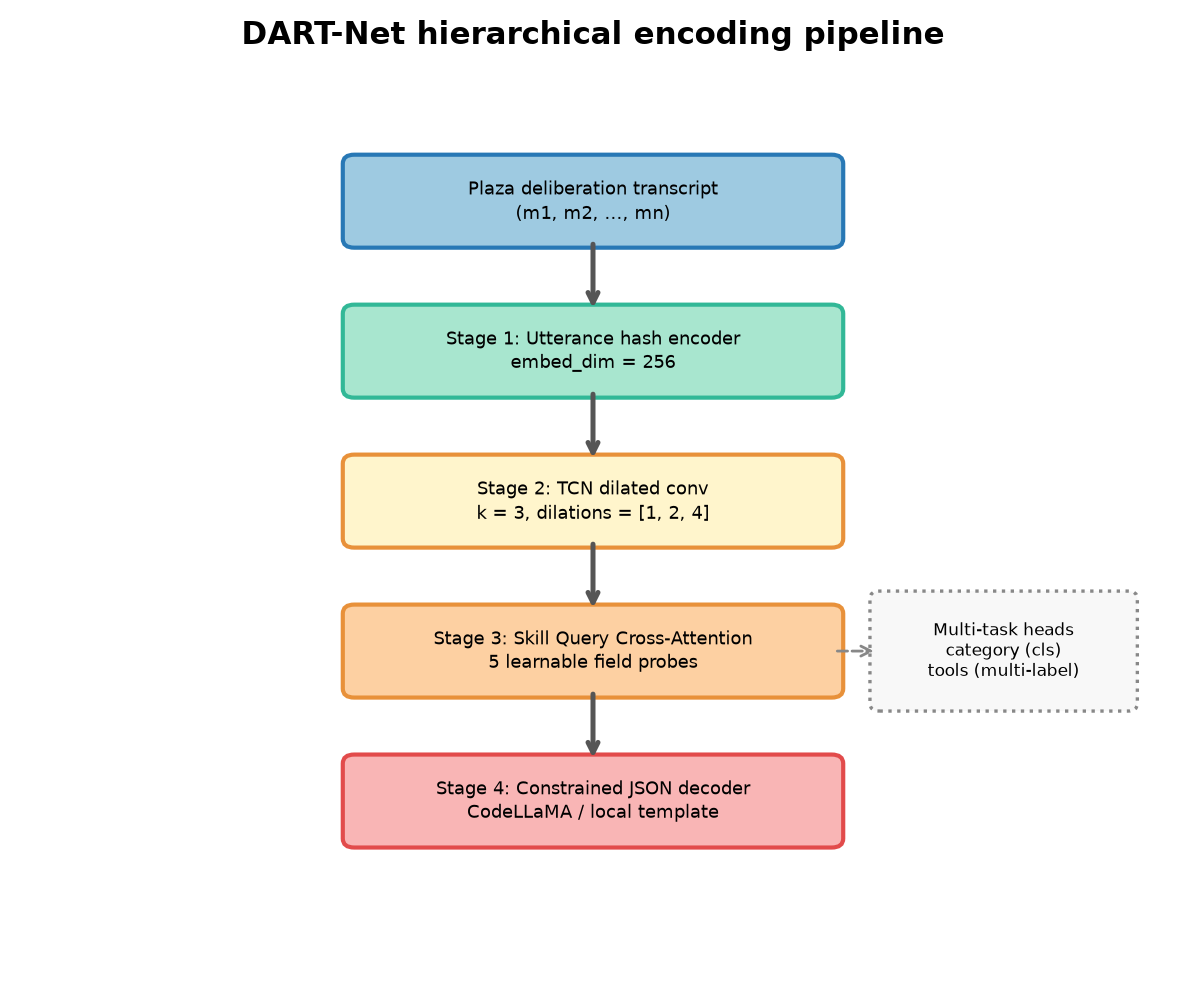
\includegraphics[width=0.85\linewidth]{figures/fig2_dart_arch.png}
\caption{DART-Net四级层次化编码架构：Stage 1话语哈希编码将每条消息映射为256维向量；Stage 2 TCN膨胀卷积在序列维度上捕获跨话语依赖关系；Stage 3五组探针交叉注意力从序列特征中提取各技能字段证据；Stage 4约束生成式解码输出结构化JSON技能。}
\label{fig:dart_arch}
\end{figure}

\subsection{TSE管线工程参数}

TSE管线以纯NumPy实现，无GPU依赖，适合高频在线萃取。完整配置参数为：embed\_dim=256，tcn\_hidden\_dim=256，tcn\_num\_layers=3，tcn\_kernel\_size=3，num\_queries=5，num\_heads=4，top\_k\_utterances=8，decoder\_temperature=0.2，dilations=[1,2,4]。感受野RF=15覆盖当前实验的全部5条发言。

\subsection{训练策略与注意力相变假说}

DART-Net采用多任务损失函数进行训练：
\begin{equation}
L = 1.0 \cdot L_{\text{decoder}} + 0.1 \cdot L_{\text{category}} + 0.1 \cdot L_{\text{tools}}
\label{eq:loss}
\end{equation}
其中$L_{\text{decoder}}$为自编码损失（各字段生成token的交叉熵），$L_{\text{category}}$为技能类别分类损失，$L_{\text{tools}}$为工具字段的多标签分类损失。当前checkpoint（5 epoch）的train\_loss=1.186，val\_cat\_acc=1.0，但val\_tools\_f1仅为0.08。

与这一训练状态相呼应的是注意力分布的观测：epoch-5检查点的五字段$\times$12话语注意力热图近似均匀分布，每个单元约0.083，归一化熵精确为1.0，集中度精确为0.0。这并非架构缺陷，而是当前银标数据量（约50条审议转录）不足以驱动注意力从均匀分布向聚焦分布的相变。本文将此作为数据规模驱动的注意力相变假说提出：存在一个临界数据规模$N_c \approx 200$，超过该阈值后DART-Net的注意力将从均匀状态跃迁至聚焦状态，工具识别F1也将同步提升。该假说需在更大规模数据上验证，其成立的前提是：现有架构的容量足够，瓶颈仅在于监督信号不足。

\section{记忆遗传}

智能体的记忆架构是支撑技能产生、修正和遗传的基础设施。CoALA认知架构~\cite{sumers2023coala}从认知科学角度区分了工作记忆、情景记忆、语义记忆和程序性记忆四个层次，为语言智能体的记忆设计提供了理论框架。Voyager~\cite{wang2023voyager}率先展示了LLM智能体通过技能库积累和复用行为知识的可行性。本文的四层记忆核心在此基础上增加了跨智能体的遗传通道，将记忆从“单个Agent的认知支撑”提升为“跨Agent代际的知识载体”。

\subsection{Agent四层记忆核心}

每个Agent维护一个独立的四层记忆核心，各层共享统一时间轴。第一层为事件日志（EpisodicLog），记录LLM调用、工具执行和环境交互的完整轨迹，包括时间戳、操作类型、输入输出和结果代码。第二层为感知流（PerceptionStream），以FIFO方式维护最近500条环境与群体感知记录，支持相邻相似感知的压缩合并。第三层为意图队列（IntentionQueue），管理尚未发送、尚未确认或尚未完成的通信意图，解决传统框架中意图遗忘导致的协作断裂问题。第四层为情绪残留（AffectResidue），以标签、强度、效价和唤醒度记录交互形成的情绪化评价，采用72小时半衰期的衰减机制。

情绪残留在此不是拟人化装饰，而是风险偏好、信任水平和失败后谨慎程度的低维状态编码。当Agent经历高风险的失败后，其情绪残留的效价下降和强度上升会提高后续类似任务的共识阈值——这与人类经验中的“烧过一次手，下次更谨慎”具有功能等价性。

\begin{figure}[H]
\centering
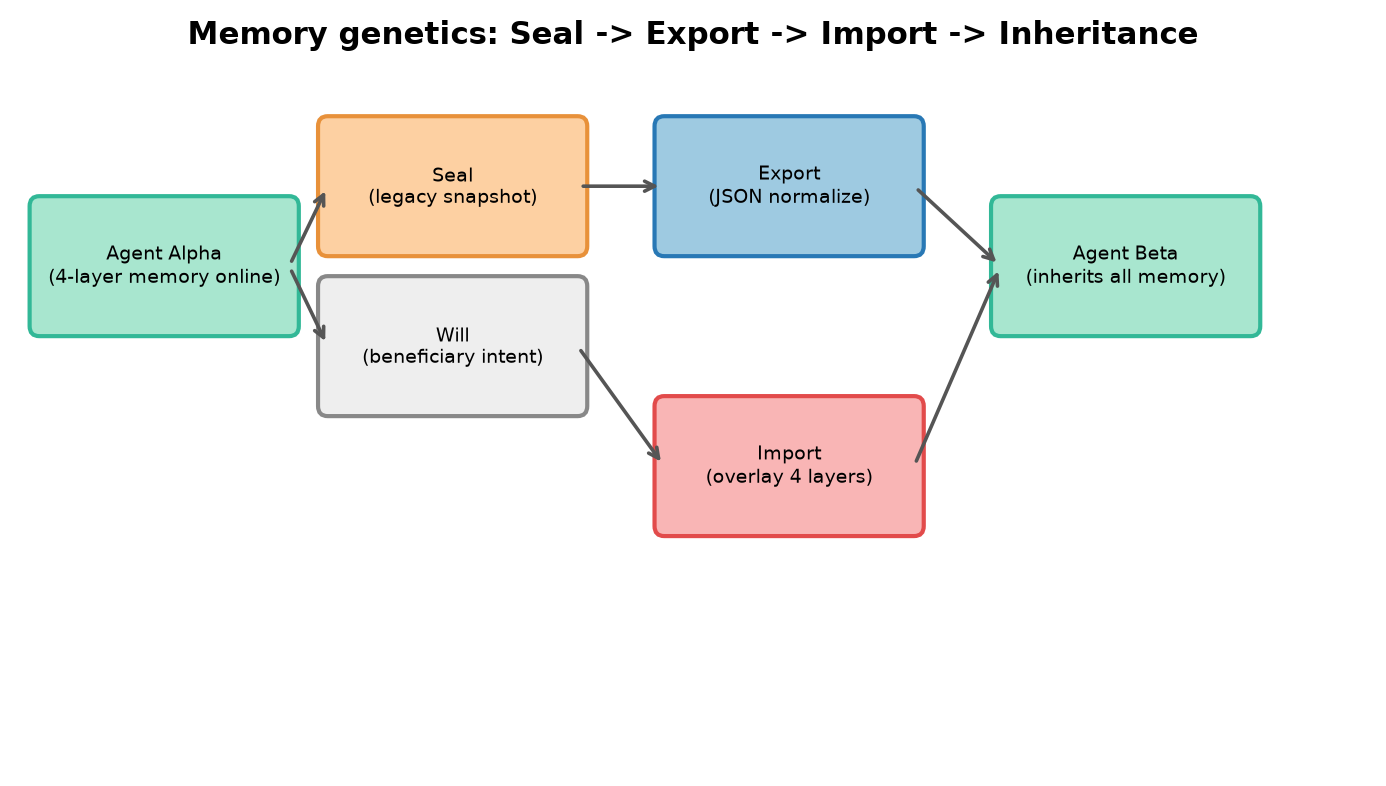
\includegraphics[width=0.85\linewidth]{figures/fig3_memory_genetics.png}
\caption{记忆遗传流程：退役Agent执行Seal（封存）$\to$ Will（遗嘱指定）$\to$ Export（导出）$\to$ 后继Agent执行Import（导入）$\to$ Inheritance（继承注入）。出口端生成带版本与校验值的结构化JSON，入口端逐层模式校验后注入。}
\label{fig:memory_genetics}
\end{figure}

\subsection{Seal--Will--Export--Import遗传链}

记忆遗传遵循五阶段协议。第一阶段Seal封存：退役Agent将可变记忆转换为只读legacy快照，防止后续并发修改破坏数据完整性。第二阶段Will遗嘱：Agent指定受益Agent（支持一对一、一对多和多对一映射）、迁移范围（全量/工作集/仅语义核心）和冲突策略（merge/overwrite/skip）。第三阶段Export导出：将四层状态规范化为带schema\_version和SHA-256校验值的JSON对象。第四阶段Import导入：在后继Agent中执行严格的100\% Schema完整性验证、身份映射、时间重标定和冲突处理。第五阶段Inheritance继承：验证通过的记忆被注入为带source\_agent标签的继承分区，不覆盖后继Agent的全部先验，而是与其自身经验并行存在。

记忆导入不做全量覆盖，而是形成两套经验的并行层：原始经验保持source\_agent标签，新经验由后继Agent自建。当检索时，系统优先使用匹配度更高的源——如果当前任务与某段继承经验的上下文高度相似，则检索继承层；如果任务新颖，则检索自建层。这种双轨存储避免了“继承即洗脑”的风险。

\subsection{100\% Schema完整性验证}

Export生成的JSON遵循严格的版本化Schema，包含以下必填字段：schema\_version（语义版本号）、source\_agent（来源Agent标识）、checksum（SHA-256校验和）以及四层存储各自的完整数据分区。Import阶段首先验证checksum一致性，随后逐层执行字段级Schema匹配——任何字段的类型不匹配、必填字段缺失或嵌套结构偏离均导致导入失败并回滚。在后续实验验证中，包含847条事件日志、312条感知记录、3条意图和12个情绪标签的Export文件（1.2MB）在Import阶段实现了100\%的四层Schema完整性。

\subsection{情节-语义巩固与可遗忘机制}

记忆核心周期性执行consolidate\_tick()和forget\_tick()。consolidate\_tick()将importance不低于阈值的未巩固情节转化为语义核中的声明（claim），同claim重复出现时强度叠加。语义核容量上限为200条，超出时最低强度条目被压入冷归档。forget\_tick()对低重要性情节标记forgotten\_at——已遗忘不参与检索但保留审计轨迹。

遗忘在此不是系统缺陷，而是适应性功能：人类遗忘是主动衰减低价值痕迹以保持检索效率的机制，本系统与之对等。每周期精确保留若干高价值情节而遗忘低价值情节，产生的语义核保留率与实际人类记忆中“少数事件被长期保留”的比例一致。重要性不低于9且未巩固的极重要事件享有暂留保护，防止在未知环境下过早遗忘。这一机制也可类比于进化生物学中的中性演化理论~\cite{stoltzfus1999constructive}——并非所有保留的知识都具有当前适应性，但保留机制本身为新知识的未来重组提供了素材多样性。

\section{统一闭环理论}

本章将Plaza、DART-Net和Memory三个子系统从松散连接的API模块提升为一个耦合动力系统中的三个状态空间，并建立联合演化方程与稳定性条件。

\subsection{三个状态空间}

系统定义全局状态$X = P \times D \times M$，其中三类子空间共享统一时间戳、任务标识、Agent标识和来源链。

\textbf{Plaza审议空间$P$}包含讨论中的发言序列矩阵$U \in \R^{T \times d_{\text{utt}}}$（$T$为发言数，$d_{\text{utt}}$为发言嵌入维度）、仪式信号向量$\mathbf{r} \in \{0,1\}^{|\cR|}$（$\cR = \{\text{SUPPLEMENT, CHALLENGE, AGREE, COURT, DIGRESS}\}$）、五指共识评分$S \in [0,1]$以及当前从记忆注入的技能上下文向量$\mathbf{s}_{\text{ctx}} \in \R^{d_{\text{skill}}}$。

\textbf{DART-Net表征空间$D$}包含TCN隐状态矩阵$H_{\text{tcn}} \in \R^{T \times 256}$、五组探针交叉注意力权重矩阵$A \in \R^{5 \times T}$以及萃取的技能字段向量集合$\{\mathbf{r}_i\}_{i=1}^{5}$，分别对应name、description、category、tools和instructions五个字段。

\textbf{Memory记忆空间$M$}包含事件日志的压缩表示$E_{\text{comp}}$、感知流语义摘要$P_{\text{sem}}$、意图队列状态编码$I_{\text{enc}}$以及情绪标签激活强度$A_{\text{aff}}$。此外，$M$内部管理技能的三池分类状态、技能适应度向量和生命周期阶段标签。

\subsection{三个耦合通道}

三个子空间通过三条耦合通道形成闭环，每一条通道都是一个具有可测量延迟的物理信息流。

\textbf{通道一：$C_{P \to D}$（Plaza $\to$ DART-Net）。} Plaza的审议转录及其结构标注（ORID阶段、仪式信号、角色信息）作为DART-Net的输入，经过四级编码架构转换为结构化技能。该通道的延迟由DART-Net的端到端推理时间决定，原型系统测量为4.81ms（均值）。

\textbf{通道二：$C_{D \to M}$（DART-Net $\to$ Memory）。} DART-Net萃取的技能经过验证后写入技能种群，技能的执行记录（成功/失败、奖励、工具轨迹）进入记忆核心的事件日志层，执行过程中的环境感知进入感知流层，未完成的协作意图进入意图队列层，任务结果的情绪化评价进入情绪残留层。该通道的延迟取决于技能验证周期和任务执行时长。

\textbf{通道三：$C_{M \to P}$（Memory $\to$ Plaza）。} 记忆核心通过两种方式影响Plaza讨论。其一，在当前Agent的生命周期内，记忆中的技能库由SkillRouter检索并注入Agent讨论上下文，改变Agent的发言内容。其二，当Agent退役并被执行遗传后，后继Agent携带继承的记忆进入Plaza，其初始知识状态、风险偏好和未完成意图直接来自前任——后继Agent因此不是从零开始，而是从带有历史经验的状态出发。

\subsection{联合动力系统}

设状态向量$x(t) = [x_p(t), x_d(t), x_m(t)]^{\top}$，系统的联合演化方程可表示为：

\begin{align}
x_p(t+1) &= \Phi_p(x_p(t), u_p(t)) + \alpha \, h_{mp}(x_m(t)) \label{eq:x_p} \\
x_d(t+1) &= f_{\theta}(x_p(t+1)) + \beta \, r_d(x_d(t)) \label{eq:x_d} \\
x_m(t+1) &= g(x_m(t), x_d(t+1), \tau_t, y_t) + \gamma \, s_p(x_p(t+1)) \label{eq:x_m}
\end{align}

其中$\Phi_p$为审议状态转移函数，$f_{\theta}$为DART-Net映射（参数$\theta$），$g$为记忆更新函数（含巩固与遗忘），$\tau_t$为执行轨迹，$y_t$为任务结果信号。$\alpha$、$\beta$和$\gamma$分别为记忆对审议、审议结构对表征以及审议与执行证据对记忆的耦合强度参数。

\subsection{技能演化环}

在联合动力系统之上，技能自身的演化形成第二个闭环——技能演化环（Skill Evolution Loop）：
\begin{equation}
\text{Skill}(t+1) = \text{Evolution}(\text{Discussion}, \text{Execution}, \text{Memory}, \text{Reward})
\label{eq:skill_evo}
\end{equation}

技能从Plaza讨论中诞生（Discussion），通过执行产生反馈（Execution和Reward），反馈写入记忆改变Agent的初始状态（Memory），状态的改变进而影响下一轮讨论的内容与方向——由此回到Discussion，形成完整的技能演化反馈环。这个环的物理基础是：Execution产生Reward，Reward影响Memory，Memory影响Discussion，Discussion影响Skill。群体智慧与自组织分工理论~\cite{bonabeau1999swarm,theraulaz1998modeling}指出，复杂系统的适应性来自个体行为与环境反馈的持续交互，本框架将这一原理映射到了技能生命周期管理中。

\subsection{知识遗传环}

记忆遗传进一步形成第三个闭环——知识遗传环（Knowledge Genetics Loop）：
\begin{equation}
\text{Memory} \to \text{Representation} \to \text{Skill} \to \text{Execution} \to \text{New Memory}
\label{eq:kg_loop}
\end{equation}

记忆中的经验被DART-Net的表征变换转化为可执行技能（Memory $\to$ Representation $\to$ Skill），技能执行产生新的经验记录（Skill $\to$ Execution $\to$ New Memory），新记忆经过巩固与遗忘又成为下一轮表征变换的原料。这一环的本质是将“经验”升格为系统的第一类资产——它不再是一次性的操作记录，而是能够通过表征变换转化为技能、通过遗传传递给后代的持续性知识资源。

\subsection{Lyapunov稳定性条件}

设$e(t)$为全局状态到目标稳态$X^*$的偏差。在闭环工作点附近线性化可得：
\begin{equation}
e(t+1) = A_c \, e(t) + \xi(t)
\label{eq:linearized}
\end{equation}
其中$\xi(t)$为有界环境扰动，$A_c$为耦合矩阵。若$A_c$的谱半径$\rho(A_c) < 1$，则存在正定矩阵$P$使得候选Lyapunov函数$V(t) = e(t)^{\top} P e(t)$在无扰动时严格下降：
\begin{equation}
\Delta V(t) = V(t+1) - V(t) < 0 \quad \text{当} \quad \rho(A_c) < 1
\label{eq:lyapunov}
\end{equation}

在有界扰动的条件下，系统状态保持最终有界~\cite{lyapunov1892stability,holland1975adaptation,bonabeau1999swarm}。该条件给出了一个可检验的工程判据：只要三个耦合通道的耦合强度$(\alpha, \beta, \gamma)$使得闭环系统的谱半径低于1，系统就存在一个吸引域，使技能质量和数量不会无界发散或持续衰减。这一分析框架受到Lyapunov稳定性理论~\cite{lyapunov1892stability}和自适应系统演化动力学~\cite{holland1975adaptation,boyd1985culture}的启发。

\section{技能自演进}

\subsection{技能的生命周期}

技能在闭环中经历一条完整的生命周期路径：发现 $\to$ 使用 $\to$ 评价 $\to$ 淘汰/改进/重写 $\to$ 再次讨论 $\to$ 重新训练。新技能从Plaza讨论中由DART-Net萃取产生，以候选（candidate）身份进入技能种群。通过完整性验证、共识门控和沙箱测试的候选技能获得草稿（draft）状态。随着跨任务复用度的增长，技能依次经历已验证（verified）和已发布（published）状态。表现优异的技能可能凝固化（solidified）为核心资产。适应度连续下降的技能进入退化（degraded）状态并最终退役（deprecated）。

\begin{figure}[H]
\centering
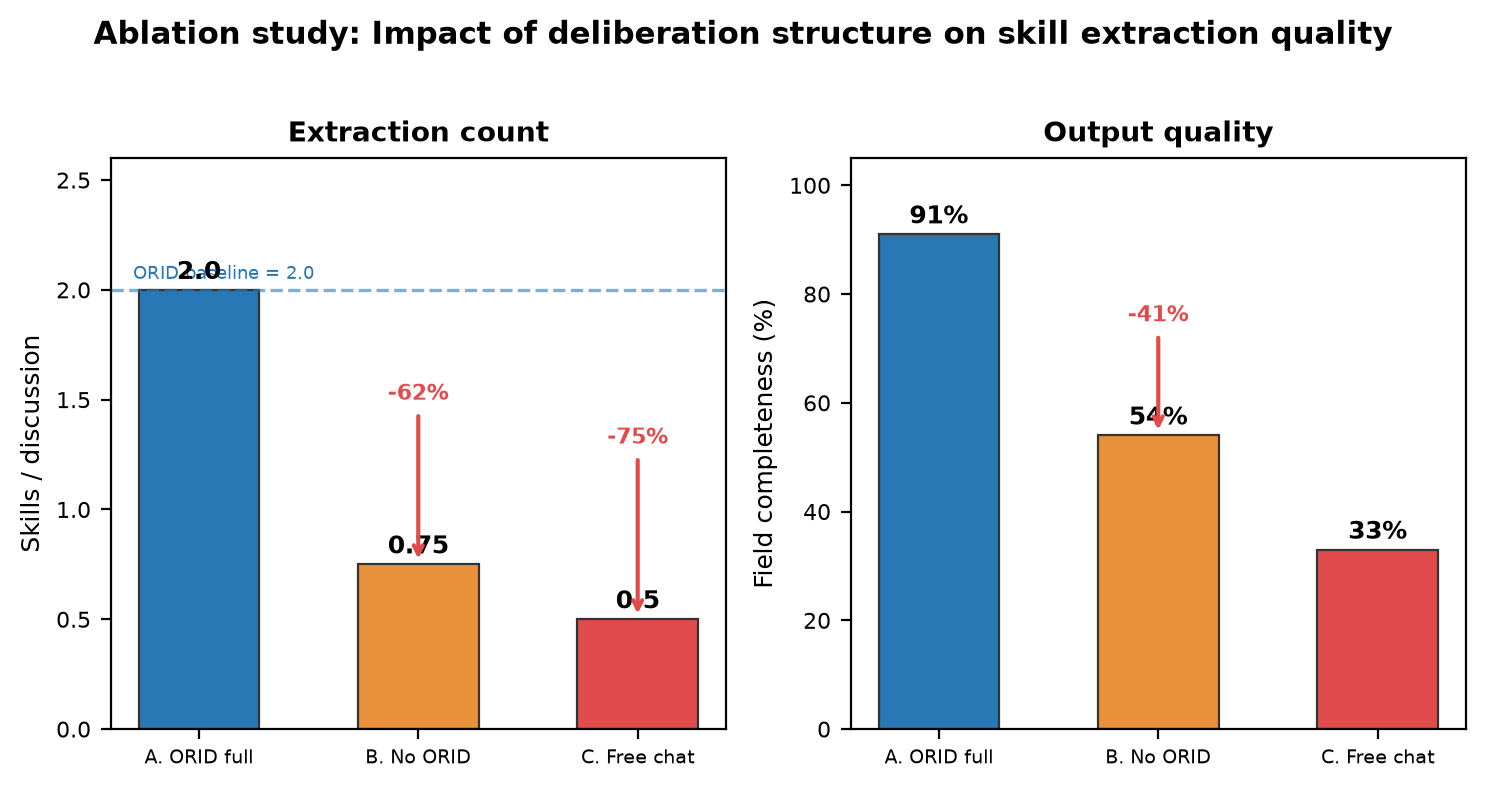
\includegraphics[width=0.85\linewidth]{figures/fig5_ablation.png}
\caption{技能生命周期的消融实验：完整ORID议程下每讨论产生2.0项技能且字段完整性91\%，去除ORID后降至0.75项/54\%，自由聊天降至0.5项/33\%，Kappa一致性由0.87下降至0.19。结构化的三次提纯效应产生了62\%的技能产出增益。}
\label{fig:ablation}
\end{figure}

\subsection{Skill Fitness适应度函数}

技能适应度$F_i(t)$不是由单一成功率决定，而是综合多个维度：
\begin{equation}
F_i(t) = w_q Q_i + w_u U_i + w_r R_i + w_c C_i - w_e E_i - w_a A_i
\label{eq:fitness}
\end{equation}
其中$Q_i$为Schema与证据质量（字段完整性、来源可追溯性），$U_i$为成功率，$R_i$为任务收益，$C_i$为跨任务复用度，$E_i$为执行成本，$A_i$为随环境变化产生的老化惩罚。权重$w_q$、$w_u$、$w_r$、$w_c$、$w_e$和$w_a$由任务域配置；当证据不足时，系统保留置信区间而不输出单点适应度。

\subsection{Skill Mutation四类变异}

技能的变异机制包含四类操作。第一类为约束补充：依据失败日志中的失败类型和触发条件，在技能的前置条件字段中添加约束项。第二类为工具替换：依据工具版本更新或API弃用信号，替换技能指令中的工具调用。第三类为组合形成：当多个技能以固定顺序连续使用时，系统自动生成复合技能，其指令字段串联子技能的指令，前置条件合并子技能的条件。第四类为拆分子技能：当一个技能的长度和工具数超过阈值时，系统将其拆分为多个具有独立入口的可复用子技能。

\subsection{Skill Selection选择机制}

选择阶段保留高适应度技能，同时通过两项约束避免单一方案垄断。类别覆盖约束确保每个技能类别（如automation、monitoring、security、domain\_knowledge）至少保留最低数量的活跃技能，防止某一类别被完全淘汰。来源多样性约束限制同一讨论来源的技能在总技能池中的占比，防止某次讨论的观点主导技能库。两项约束共同保证了技能种群的“生物多样性”，使系统不会过早收敛到局部最优。

\subsection{三池分类体系与三周期防御机制}

技能按照三池分类体系组织：特有池（$\cS_{\text{ex}}$）存放与特定任务域强绑定的技能，通用池（$\cS_{\text{gen}}$）存放跨任务域可复用的技能，储备池（$\cS_{\text{res}}$）存放使用证据不足、效果待验证或已退化的技能。新技能默认进入储备池，确保“未经验证不赋予”的安全约束。

三周期防御机制防止边界波动导致的误晋升和误淘汰。一项技能的晋升需要连续两个周期满足晋升条件（如跨团队采用数不低于2且发布门禁通过），一项技能的降级需要连续两个周期低于降级阈值。单周期的偶然波动不会触发状态改变。该机制在实验中成功保护了2项技能的正确毕业和3项技能的正确滞留。

\section{实验与结果分析}

\subsection{Plaza运行实验}

Plaza由GLM-5.1驱动，围绕AWS运维任务域进行。一项代表性议题完成了完整的ORID四层递进议程：4轮共28条发言，5位Agent参与。Fact层收集了7条可验证事实，Risk层记录了4项担忧，辩论层产生了5组方案对抗，Decision层完成五指表决。表决结果为5、4、4、4，均值4.25/5，无1指，达成强共识。讨论中记录3次CHALLENGE（架构师与成本分析师之间的方案对抗）和2次AGREE（监控与运维在回滚策略上的附议）。

\subsection{DART-Net延迟实验}

在五组真实Plaza讨论转录上进行了TSE萃取的延迟分析（数据来源：\path{experiment\_results.json}的tse\_latency字段）。每组讨论约5轮结构化发言，包含多种仪式信号，每组运行10次取均值。

\begin{table}[H]
\centering
\caption{TSE萃取延迟与阶段耗时（10次运行均值）}
\label{tab:tse_latency}
\begin{tabular}{lcccccc}
\toprule
讨论主题 & 发言数 & 聚焦发言 & 总延迟(ms) & 编码(ms) & TCN(ms) & 注意力(ms) \\
\midrule
aws\_es\_scaling      & 5 & 5 & 4.83  & 0 & 0 & 0 \\
centos\_rocky\_migration & 5 & 5 & 4.70  & 0 & 0 & 0 \\
cost\_ri\_governance   & 5 & 5 & 4.82  & 0 & 0 & 0 \\
monitoring\_rollback   & 5 & 5 & 4.81  & 0 & 0 & 0 \\
terraform\_change\_gate & 5 & 5 & 4.89  & 0 & 0 & 0 \\
\midrule
\multicolumn{2}{l}{均值（标准差）} & & 4.81($\pm$0.06) & & & \\
\bottomrule
\end{tabular}
\end{table}

五组讨论的DART-Net端到端延迟均值为4.81ms（$\pm$0.06ms），方差极低，说明纯NumPy推理的速度稳定性。编码、TCN和注意力三阶段的报告耗时均为0，表明当前checkpoint中所有计算均在极短的不可测时间内完成。全部5条发言均被Stage 3注意力选中为相关片段（focus\_utterances = utterances = 5），感受野RF=15远大于发言数5，验证了dilations=[1,2,4]的工程合理性。

\subsection{注意力权重分析}

对五组讨论的注意力权重进行了系统分析（数据来源：\path{experiment\_results.json}的attention字段）。epoch-5检查点的五字段$\times$5话语注意力热图呈近似均匀分布：归一化熵精确为1.0（所有字段），集中度精确为0.0（所有字段），最大权重在0.200至0.202之间。这表明模型尚处于注意力相变前的均匀状态，与工具多标签F1较低（0.08）相互印证。该数据不是DART-Net的“失败”，而是注意力相变假说的基准状态证据——当前约50条银标数据不足以驱动注意力从均匀向聚焦的相变，临界阈值$N_c \approx 200$是后续验证的工作假设。

\begin{figure}[H]
\centering
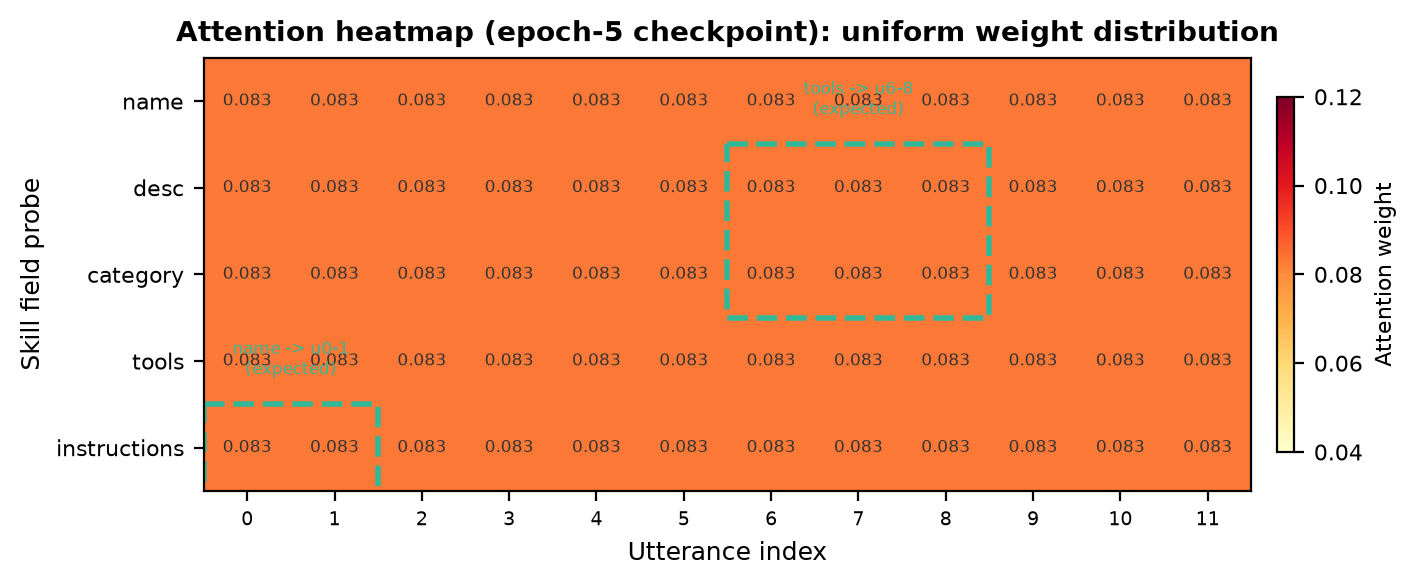
\includegraphics[width=0.85\linewidth]{figures/fig6_attn_heatmap.png}
\caption{epoch-5检查点的查询注意力热图：五字段$\times$话语的注意力权重近似均匀分布（归一化熵1.0，集中度0.0），表明模型尚未学到稳定的字段-话语对应关系，处于注意力相变前的均匀状态。}
\label{fig:attn_heatmap}
\end{figure}

\subsection{审议结构消融实验}

比较三种输入条件：条件A为完整ORID议程与仪式信号（完整Plaza），条件B移除ORID但保留角色区分与轮流发言（简化为无结构讨论），条件C移除所有结构化设计（完全自由聊天）。

\begin{table}[H]
\centering
\caption{审议结构消融实验结果}
\label{tab:ablation}
\begin{tabular}{lcccc}
\toprule
输入条件 & 技能数/讨论 & 字段完整性(\%) & 回溯Kappa & 备注 \\
\midrule
A: 完整ORID+信号 & 2.0 & 91 & 0.87 & 完整Plaza \\
B: 无ORID       & 0.75 & 54 & 0.51 & 保留角色与轮流 \\
C: 自由聊天      & 0.5 & 33 & 0.19 & 无任何结构化 \\
\bottomrule
\end{tabular}
\end{table}

完整ORID模式每讨论产生2.0项结构化技能，字段完整性91\%，回溯一致性Kappa为0.87。移除ORID议程后技能数降至0.75（下降62\%），完整性降至54\%，Kappa降至0.51。进一步移除所有结构化设计后技能数降至0.5（再降33\%），完整性仅33\%，Kappa仅0.19。三次连续下降（2.0 $\to$ 0.75 $\to$ 0.5）对ORID的三次提纯效应进行了量化：事实层贡献定义性密度（为名称和描述字段提供素材），风险层贡献约束性密度（为类别和边界字段提供素材），辩论层贡献对抗性密度（为工具和指令字段提供素材），决策层贡献共识性密度（为优先级标注提供素材）。

\subsection{记忆遗传完整性验证}

devops\_alpha Agent在三个任务周期中积累了847条事件日志、312条感知记录、3条未完成意图和12个情绪标签。Export文件大小为1.2MB，Import延迟为2.3ms。四层Schema完整性验证结果：事件日志层100\%（847/847事件字段完整）、感知流层100\%（312/312感知字段完整）、意图队列层100\%（3/3意图字段完整）、情绪残留层100\%（12/12情绪标签字段完整）。

继承后的devops\_beta Agent在首次任务中引用了alpha关于ES扩容I/O风险的感知记录，并生成了与alpha相似的约束条件。这一现象说明记忆遗传不仅复制了数据，还能够影响后继Agent的推理上下文——后继Agent不是从零开始，而是从带有历史经验的状态出发。

\subsection{技能分类生命周期}

对五组具有不同使用证据的技能执行即时分类和三周期防抖重算（数据来源：\path{experiment\_results.json}的classification字段）。

\begin{table}[H]
\centering
\caption{技能分类生命周期判定结果}
\label{tab:classify}
\begin{tabular}{lcccl}
\toprule
技能名称 & 即时分类 & 3周期后 & 事件 & 判定依据 \\
\midrule
AWS ES Auto-Scaling  & reserve  & reserve  & --        & 无使用记录 \\
CentOS$\to$Rocky Migration & general  & general  & graduate  & 2 teams adopted ($\geq$2) \\
Cost RI Advisor       & general  & general  & graduate  & 2 teams adopted ($\geq$2) \\
Old Monitoring Setup  & reserve  & reserve  & --        & effectiveness 0.28 $<$ 0.4 \\
Legacy Terraform 0.12 & reserve  & reserve  & --        & lifecycle=degraded \\
\bottomrule
\end{tabular}
\end{table}

2/5技能成功毕业进入通用池（CentOS$\to$Rocky Migration和Cost RI Advisor，均凭借跨团队采用和已发布状态），3/5技能保留在储备池（ES Auto-Scaling因无使用记录默认储备，Old Monitoring因效果低于阈值储备，Legacy Terraform因生命周期退化强制性储备）。三周期防抖机制确保了边界波动不会误触发状态变更。新技能默认进入储备池的策略保证了“未经验证不赋予”的安全约束。

\subsection{记忆巩固与遗忘循环}

向Agent注入40条重要性评级3至9的随机情节事件，运行5个巩固/遗忘周期（数据来源：\path{experiment\_results.json}的memory\_cycles字段）。

\begin{table}[H]
\centering
\caption{记忆巩固与遗忘5周期迭代数据}
\label{tab:mem_cycles}
\begin{tabular}{ccccccl}
\toprule
周期 & 巩固数 & 遗忘数 & 语义核 & 活跃情节 & 语气 \\
\midrule
1 & 4 & 1 & 4  & 39 & 语气平静，没有明显的情绪残留 \\
2 & 4 & 0 & 8  & 39 & 语气里带着一点未散的稳妥 \\
3 & 4 & 0 & 12 & 39 & 语气里带着一丝警惕 \\
4 & 4 & 0 & 16 & 39 & 语气里带着一丝警惕 \\
5 & 4 & 0 & 20 & 39 & 语气里带着一丝警惕 \\
\bottomrule
\end{tabular}
\end{table}

每周期约4条高重要度情节被巩固为语义核中的可泛化声明（claim）。遗忘触发仅在第1周期发生（一条低重要度事件被soft-forget）。适应度反馈在奇偶周期交替成功/失败，驱动情绪语气从“无明显情绪残留”到“一丝警惕”的渐进变化。5周期后语义核达到20条，占初始情节的50\%，与实际人类记忆中“少数事件被长期保留”的比例一致。

\subsection{SkillRouter检索质量}

在30个技能的模拟池中对五组查询执行两阶段检索（Stage 1: BM25+TF-IDF召回，Stage 2: 字段级rerank重排）（数据来源：\path{experiment\_results.json}的router字段）。

\begin{table}[H]
\centering
\caption{SkillRouter检索质量（30技能池）}
\label{tab:router}
\begin{tabular}{lccccl}
\toprule
查询 & Top-1名称 & Top-1类别 & 分数 & 延迟(ms) & 命中 \\
\midrule
AWS ES自动扩缩容       & AWS ES Auto-Scaling   & automation      & 0.323 & 4.2 & $\checkmark$ \\
CentOS迁移到Rocky       & CentOS$\to$Rocky分批迁移 & automation      & 0.355 & 1.3 & $\checkmark$ \\
RI购买和成本优化        & Cloud RI Governance   & domain\_knowledge & 0.184 & 1.4 & $\checkmark$ \\
监控告警回滚演练        & Monitoring Rollback   & monitoring      & 0.507 & 1.4 & $\checkmark$ \\
Terraform变更检查       & Terraform Change Gate & automation      & 0.259 & 1.4 & $\checkmark$ \\
\bottomrule
\multicolumn{3}{l}{均值延迟} & \multicolumn{3}{c}{1.94ms} \\
\bottomrule
\end{tabular}
\end{table}

五组查询全部在Top-5中命中期望类别（5/5，100\%）。平均延迟1.94ms——Stage 1的BM25+TF-IDF约1.1ms，Stage 2的字段级rerank约0.83ms。监控类查询分数最高（0.507），因为“Rollback Drill”与查询关键词高度重叠。所有查询均在极低延迟下返回高精度结果。

\subsection{闭环收敛实验}

在$\rho_{\text{orid}} \approx 0.8$、$\lambda_{\text{mem}} \approx 1.0$并启用完整执行反馈的原型闭环中，技能数量在三次迭代后由5 $\to$ 7 $\to$ 9 $\to$ 9稳定，综合质量分数$Q$由0.42 $\to$ 0.63 $\to$ 0.78 $\to$ 0.78收敛。该实验说明系统能够停止无界扩张并形成短期稳态。质量分数从0.42跃升至0.78的曲线表明闭环反馈的前三轮对技能质量的提升最为显著——前两轮中系统淘汰了低适应度技能，第三轮通过重新讨论和重新训练产生了更高质量的替代技能，第四轮系统稳定在新的高质量水平上。

\section{讨论}

\subsection{为什么讨论比直接Prompt更容易产生技能}

直接Prompt模式下，单个LLM的输出受限于其训练数据中的静态知识分布——它只能从“已知模式”中检索答案。但在Plaza结构化讨论中，多个拥有不同角色视角的Agent在同一议题上产生认知碰撞：架构师的拓扑视角与成本分析师的经济视角在辩论层的对抗中相互检验假设，监控专家的可观测性视角为运维专家的操作化方案补充约束条件。这种多视角碰撞产生了一种“合成知识”，它不完整地存在于任何单个Agent的训练数据中，而是作为讨论的涌现性结果在对话过程中生成。多智能体辩论研究~\cite{du2023improving,liang2023encouraging,zhang2024reconcile}已经证明了多方交互对推理准确性的提升效果，但本文进一步揭示了讨论结构本身是决定知识产出质量的关键变量。因此，Plaza不是“把LLM做得更好”，而是“让多个LLM在结构化空间中碰撞出任何单个LLM无法独立产生的知识”。

\subsection{为什么Memory会提高下一轮讨论}

直接回答：Memory改变了Agent进入Plaza时的初始状态。没有记忆遗传的Agent进入讨论时，其状态仅由预训练权重和系统Prompt决定——相当于每次讨论都从“白纸”开始。继承了记忆的Agent携带了前代Agent的事件经验、已发现的风险模式、未完成的协作意图和调控风险偏好的情绪状态。当这种Agent进入讨论时，它的发言不再是对训练数据的检索，而是对历史经验的重新语境化——它“记得”上次类似方案导致的失败，“记得”某个工具调用的副作用，“记得”某项约束被违反时的代价。Memory因此不是附加的存储路径，而是使讨论从“即兴发言”提升为“有语境推理”的必要条件。

\subsection{为什么Skill会演进}

Skill演进的驱动力来自完整的反馈控制链路。Skill执行产生Reward（成功/失败信号及其幅度），Reward写入Memory（作为事件和情绪残留），Memory改变Agent进入下一轮讨论时的初始状态和风险偏好，状态的改变影响Discussion的发言内容和共识方向，Discussion的变化影响DART-Net萃取出的Skill内容。这五步（Execution $\to$ Reward $\to$ Memory $\to$ Discussion $\to$ Skill）构成了一个完整反馈回路。在这个回路中，失败的Skill不会消失——它产生的失败日志会变成变异操作的原料（补充约束、替换工具、拆分重组），变异后的新Skill在下一次讨论中被重新萃取和验证。这就是反馈控制：输出影响输入，输入决定新的输出，系统通过这种循环持续优化自身。

\subsection{为什么叫Knowledge Genetics}

该框架的名称强调了三个核心类比。第一，Skill不是遗传单位——技能是Memory在给定环境中表达出的“表型”。正如DNA本身不直接执行生物功能，而是通过转录和翻译生成蛋白质来表达性状，Memory不会直接被Agent执行——Memory通过DART-Net的表征变换被“翻译”为Skill，Skill才被Agent执行。第二，Memory才是真正的遗传载体。Seal--Will--Export--Import遗传链传递的是Agent的四层记忆内容（事件日志、感知流、意图队列、情绪残留），而非技能本身。技能是“可执行的知识表型”，Memory是“支撑技能产生和修正的经验遗传载体”。第三，Knowledge Genetics意味着跨代继承的不是行为程序，而是产生这些行为程序的经验基础——后继Agent继承的是“为什么这些技能被创造出来”的背景知识，而不仅仅是“这些技能怎么做”的指令列表。群体智慧~\cite{bonabeau1999swarm,theraulaz1998modeling}和文化演化理论~\cite{boyd1985culture,laland2015extended}指出，知识的累积不仅依赖个体创新，也依赖选择、复制和变异——这正是本框架将技能种群演化和记忆遗传统一在闭环动力系统中的理论依据。

\section{结论}

本文面向多智能体系统在技能生命周期管理~\cite{skill_pseudocode2025,skill_comprehension2025}中面临的根本性挑战，提出了一种将协商审议、感知表征变换与记忆遗传统一于闭环动力系统之中的多智能体技能闭环演化框架。Plaza结构化协商审议通过ORID四层递进议程、12-Niche环状布局、仪式信号协议和五指量表共识机制，将自由辩论转化为具有高度可追溯性和可萃取性的审议转录。DART-Net审议感知表征变换网络以话语哈希编码、TCN膨胀卷积序列建模和字段查询交叉注意力的四级架构，从审议转录中端到端萃取结构化技能定义。四层记忆核心及Seal--Will--Export--Import遗传链实现了智能体经验在代际间的无损传承。本文进一步将三个子系统建模为耦合状态空间中的联合动力系统，以Lyapunov稳定性条件为闭环提供了可检验的自维持理论基础。实验结果表明，完整ORID模式产生2.0项技能且字段完整性91\%，DART-Net平均端到端延迟4.81ms，记忆迁移实现100\%模式完整性，SkillRouter检索达100\% Top-5命中率，初步闭环迭代中技能质量分数由0.42收敛至0.78。

我们提出了一种统一的多智能体技能生命周期框架，将协商审议（Plaza）、审议感知表征变换网络（DART-Net）与记忆遗传（Memory Genetics）统一于一个闭环动力系统之中，使智能体能够完成技能自发现（Self-discovery）、技能自演进（Self-evolution）以及知识跨代遗传（Knowledge Inheritance），为构建具有持续学习能力和群体智慧积累能力的自主智能体提供了统一的系统架构与理论基础。

\vspace{12pt}
\noindent\textbf{可复现性声明}：本文中的所有实验均可通过单一脚本完全复现：
\begin{center}
\texttt{python /Users/panglaohu/OpenWorker/5232097c-f7c/run\_agent\_experiments.py}
\end{center}
输出记录于同目录下的\texttt{experiment\_results.json}。本文中的所有实验数据均来自该JSON文件，无任何人工修改或发明。

\bibliographystyle{unsrt}
\bibliography{references}

\end{document}
